\part{Utilisation, production, sources de pollution et types d'environnements contamin\'es}
\setcounter{section}{0}
\section{Utilisation}
\par{
La plupart des plastiques, ayant une densit\'e assez faible sont l\'egers. Ils ont des propri\'et\'es thermiques, m\'ecaniques, \'electriques, optiques permettant d'en faire des produits \`a usages divers. Certains peuvent \^etre transparents, permettant de fabriquer des dispositifs optiques. Ils r\'esistent \`a l'action corrosive de nombreuses substances. On peut les mouler facilement dans des formes complexes, permettant d'int\'egrer diff\'erentes mati\`eres et fonctions. De plus, en vue d'am\'eliorer ou modifier certaines de leurs propri\'et\'es physiques, on peut y ajouter des mati\`eres de renforcement, des colorants, des retardateurs de flamme, des plastifiants, afin de r\'epondre aux besoins d'une application donn\'ee. Le secteur des emballages est le plus gros consommateur de plastique. Plus de 50\% des marchandises en Europe sont emball\'ees dans du plastique {\citep{Plasticseurope2}}.
}
\par{
Une part importante de l'utilisation du plastique concerne le secteur de l'emballage , mais aussi celui du b\^atiment, des transports, de l'\'electricit\'e et d'autres usages vari\'es comme le mat\'eriel de sports et de loisirs {\citep{SCF}}.
}

\begin{figure}[h]
\centering
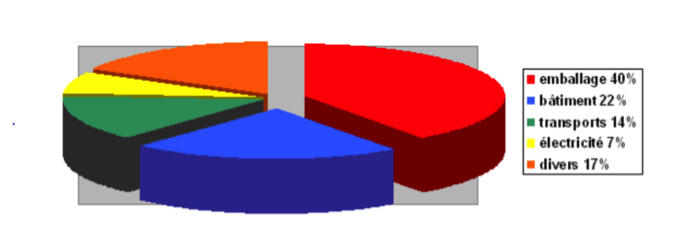
\includegraphics[scale=1]{Secteurs.png}
\caption{Consommation des mati\`eres plastiques selon les secteurs d'utilisation {\citep{SCF}}} 
\label{secteurs}
\end{figure}
\FloatBarrier

\par{
La consommation est diff\'erente selon la forme d'utilisation. Le tableau ci-dessous reprend les diff\'erents types de plastique et leurs formes d'utilisation les plus courantes:
}

\begin{table}[h]
\centering
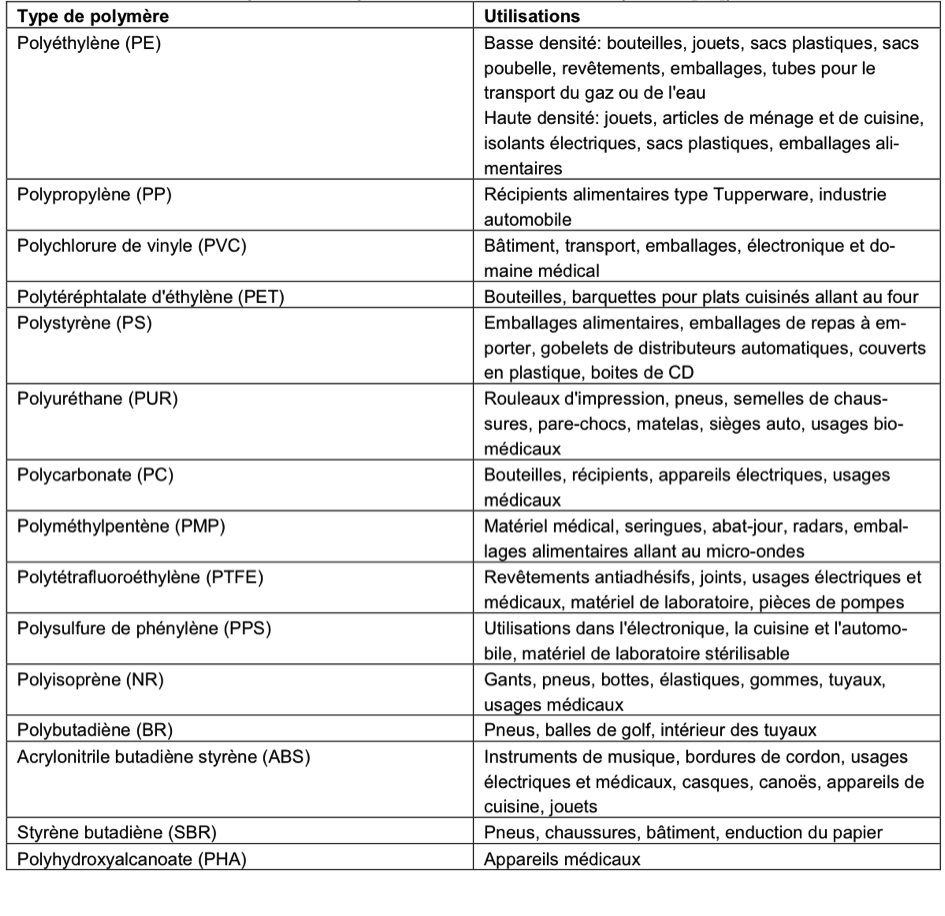
\includegraphics[scale=1]{Diffpoly.png}
\caption{Les diff\'erents types de polym\`eres et leurs principales utilisations {\citep{Schafer2015}}} 
\label{diffpoly}
\end{table}
\FloatBarrier

\section{Production du plastique}
\par{
La  quantit\'e  de  plastique  produite  dans  le  monde  est  pass\'ee de 230 \`a 322 millions de tonnes par an en dix ans {\citep{Plasticseurope}} consommant 8\% environ de la production mondiale de p\'etrole {\citep{Planetoscope}}. Le vapocraquage est un proc\'ed\'e p\'etrochimique qui consiste \`a obtenir, \`a partir d'une coupe p\'etroli\`ere telle que le naphta, des alc\`enes qui sont \`a la base de l'industrie des mati\`eres plastiques produisant ainsi le poly\'ethyl\`ene ou le polypropyl\`ene par exemple {\citep{Europetrole}}.
}

\begin{figure}[h]
\centering
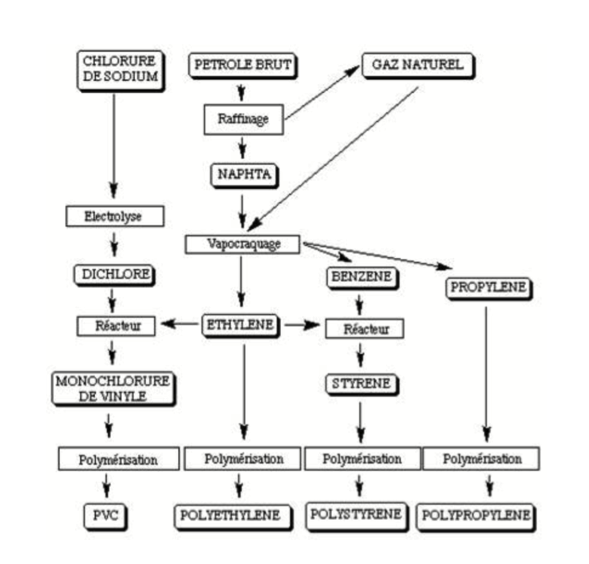
\includegraphics[scale=1]{Fabrication.png}
\caption{Modes de fabrication des principaux thermoplastiques {\citep{SCF}}} 
\label{fabrication}
\end{figure}
\FloatBarrier

\section{Sources de pollution et types d'environnements contamin\'es}
\par{
Les plastiques peuvent p\'en\'etrer dans l'environnement lors de la production, par transformation des hydrocarbures, lors de l'utilisation et du traitement des d\'echets industriels et m\'enagers.
}
\subsection{Dans les oc\'eans}
\par{
Les sources oc\'eaniques comprennent les objets perdus ou jet\'es des navires de p\^eche commerciale, ou par les plaisanciers. De m\^eme, des d\'echets plastiques peuvent provenir des plateformes p\'etroli\`eres en mer. Des pertes de fret peuvent \'egalement survenir lors de la navigation pendant les intemp\'eries ou des objets perdus lors d'un chargement ou d'un d\'echargement {\citep{lambert2014occurrence}}. La Convention MARPOL a \'et\'e adopt\'ee le 2 novembre 1973 \`a l'OMI, visant \`a pr\'evenir et \`a r\'eduire au minimum la pollution due aux navires {\citep{OMI}}.
}
\par{
Lors de leur rejet dans l'environnement, les plastiques sont transport\'es et distribu\'es dans diff\'erents types d'environnement. Les distances parcourues par un d\'echet plastique d\'ependent de sa taille et de son poids. Les mat\'eriaux l\'egers peuvent \^etre facilement transport\'es sur de longues distances, transport\'es par le vent ou par les cours d'eau jusqu'\`a s'accumuler dans les oc\'eans. Au niveau des d\'echarges \'egalement, des produits peuvent \^etre transport\'es vers la mer, en cas de fortes pr\'ecipitations {\citep{lambert2014occurrence}}. Les mati\`eres plastiques dominent les d\'ebris marins. La proportion d'articles en plastique parmi les d\'etritus augmente avec la distance des zones sources. En effet, ils sont transport\'es plus facilement que des mat\'eriaux plus denses et \'egalement parce qu'ils ont une dur\'ee de vie plus longue que d'autres mat\'eriaux qui pourraient \^etre de plus faible densit\'e {\citep{ryan2009monitoring}}. Les mati\`eres plastiques retrouv\'ees dans le milieu marin proviennent soit d'une pollution in-situ provenant des activit\'es de la mer soit par le ruissellement des rivi\`eres, les eaux us\'ees ou v\'ehicul\'ees par le vent provenant \'egalement des plages {\citep{ryan2009monitoring}}. Les d\'ebris de plastiques sont r\'epandus dans l'environnement marin mondial s'\'etendant des r\'egions polaires \`a l'\'equateur, des rivages lointains aux littoraux peupl\'es, de la c\^ote \`a la pleine mer, et jusque dans le fond des oc\'eans. Les concentrations de micro-plastiques trouv\'ees dans la banquise arctique provenant d'endroits \'eloign\'es peuvent \^etre plus importantes que celles qui ont \'et\'e observ\'ees au niveau de la surface de l'eau de mer fortement contamin\'ee comme celles du gyre du Pacifique {\citep{wang2016behaviors}}.
}

\subsection{Dans l'eau douce}
\par{
On retrouve des microplastiques \`a la surface de lacs comme c'est le cas pour les grands lacs am\'ericains et leurs rives. Il s'agit en g\'en\'eral de polystyr\`ene, de poly\'ethyl\`ene et de polypropyl\`ene. Les  fleuves  dans  leur  ensemble  sont  des  vecteurs importants  de  microplastiques  et  contribuent  ainsi  \`a  la pollution  des  mers sans que cette pollution ne repr\'esente un danger direct pour l'environnement et pour l'homme. On estime que le Rh\^one transporte chaque jour 10 kg de microplastiques vers la France {\citep{Schafer2015}}.
}

\subsection{Dans les sols}
\par{
Les sources de pollution du sol proviennent directement des d\'etritus jet\'es par terre et du d\'eversement ill\'egal des d\'echets.
}
\par{
Les d\'echets plastiques sont g\'en\'eralement collect\'es et transf\'er\'es dans des d\'echarges. Ils sont enfouis dans le sol et recouverts de terre r\'eguli\`erement. Dans les pays en d\'eveloppement, il n'existe pas toujours d'infrastructure ad\'equate ni pour le ramassage des ordures ni pour l'enfouissement au niveau de d\'echarges et les d\'ebris sont souvent souffl\'es par le vent {\citep{lambert2014occurrence}}. 
}
\par{
Des d\'ebris li\'es aux eaux us\'ees sont \'egalement une source \`a partir de laquelle les plastiques peuvent entrer dans l'environnement. Les plastiques associ\'es \`a des produits cosm\'etiques ou d'hygi\`ene corporelle sous forme de microbilles peuvent se retrouver dans le syst\`eme des \'egouts {\citep{Schafer2015}}. Les produits de plus grande taille sont g\'en\'eralement \'elimin\'es par des m\'ethodes de d\'epistage, mais ils peuvent p\'en\'etrer dans l'environnement pendant les p\'eriodes de fortes pluies provoquant des d\'ebordements des eaux us\'ees. Quant aux microbilles et \'egalement les fibres provenant des machines \`a laver, elles peuvent \'egalement passer \`a travers les proc\'ed\'es de criblage et p\'en\'etrer dans l'environnement dans les boues d'\'epuration {\citep{lambert2014occurrence}}.
 }
 \par{
Les sols peuvent \'egalement \^etre contamin\'es par des d\'echets plastiques d'origine industrielle ou agricole. Ces sources de d\'echets comprennent des technologies utilisant des billes microscopiques pour enlever la peinture ou pour nettoyer des pi\`eces de moteurs et p\'en\`etrent dans le sol par les eaux us\'ees {\citep{lambert2014occurrence}}. 
}
